\begin{ledgroupsized}[r]{120mm}
\footnotesize
\pstart
\noindent\textbf{\"{U}berlieferung:}
\pend
\end{ledgroupsized}
\begin{ledgroupsized}[r]{114mm}
\footnotesize
\pstart
\parindent -6mm
\makebox[6mm][l]{\textit{L}}Aufzeichnung: LH XXXVII 3 Bl. 88.
1 Bl. 4\textsuperscript{o}. 1 S. auf Bl. 88~r\textsuperscript{o}. Bl. 88~v\textsuperscript{o} leer.
Blatt oben und unten beschnitten; der untere abgetrennte Teil überliefert N.~65. %??037,03_089
Ein Wasserzeichen.
\\%
Cc 2, Nr. 1141
\pend
\end{ledgroupsized}
%\newpage% PR: Rein provisorisch !!!
\vspace*{8mm}
\count\Afootins=1500
\count\Bfootins=1500
\count\Cfootins=1500
\pstart%
\normalsize%
\noindent%
% [88~r\textsuperscript{o}]
[88~r\textsuperscript{o}]
Mons. l'Abb\'{e} Galin\'{e}e\protect\index{Namenregister}{\textso{Galin\'{e}e}, Ren\'{e} de Br\'{e}han de 1645-1678} me dit,
qu'on a \edtext{propos\'{e} \`{a} l'Acad\'{e}mie un Instrument,\protect\index{Sachverzeichnis}{instrument}
qui serviroit \`{a} s\c{c}auoir la  rapidit\'{e} de l'eau,
et la vistesse du chemin du vaisseau.\protect\index{Sachverzeichnis}{vaisseau}%
}{\lemma{propos\'{e} [...] vaisseau}\Cfootnote{Über ein Instrument zur Bestimmung der Str\"{o}mungsgeschwindigkeit einer Fl\"{u}ssigkeit wurde an der Pariser Akademie der Wissenschaften im Jahre 1668 berichtet. Siehe \cite{00295}B.~\textsc{de Fontenelle}, \textit{Histoire de l'Acad\'{e}mie Royale des Sciences}, Bd. I, Paris 1733, S.~73f.}}
Mais sur mer on ne s\c{c}auroit discerner la vistesse qui vient du courant\protect\index{Sachverzeichnis}{courant d'eau} de celle qui vient du vent.\pend 
\pstart 
 \begin{wrapfigure}[14]{l}{0.42\textwidth}                    
              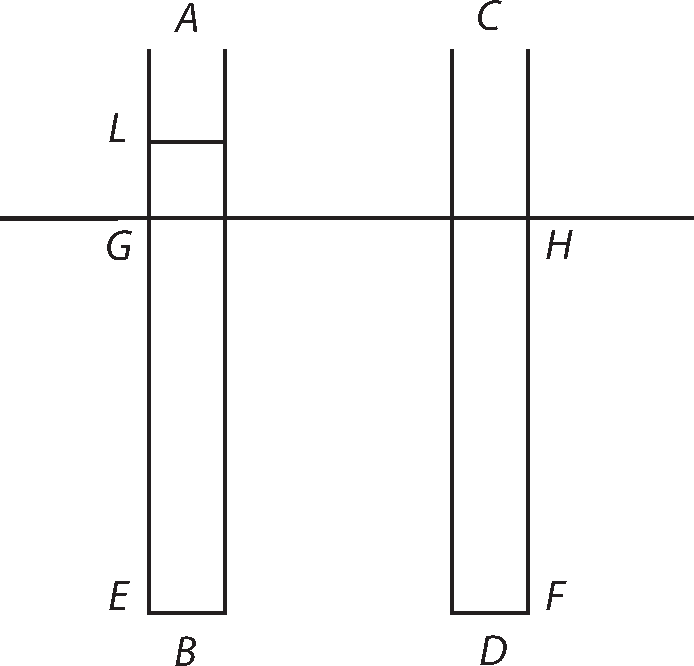
\includegraphics[trim = 0mm -2mm -5mm 0mm, clip, width=0.42\textwidth]{images/LH037,03_88r-d.pdf}
              \noindent \centering [\textit{Fig. 1}] \\
                \end{wrapfigure}
Mons. le duc de Roanez\protect\index{Namenregister}{\textso{Roanez}, Artus Gouffier de 1627-1696} me parla d'un instrument\protect\index{Sachverzeichnis}{instrument} assez joly pour s\c{c}auoir la  rapidit\'{e} de l'eau. Soyent deux tuyaux\protect\index{Sachverzeichnis}{tuyau},
$AB$, $CD$ de verre,\protect\index{Sachverzeichnis}{verre}
le courant\protect\index{Sachverzeichnis}{courant d'eau} de l'eau vient de $E$
\edtext{vers $F.$ ou $G$ vers $H.$ la fleur d'eau $G.H$}%
{\lemma{vers $F.$}\Bfootnote{%
\textbar\ ou $G$ vers $H.$ \textit{erg.} \textbar\ %
\textit{(1)}\ l'eau entre dans \textit{(2)}\ Les deux eaux \textit{(3)}\ la fleur d'eau $G.H$ \textit{L}}}
ou son niveau.
Les tuyaux\protect\index{Sachverzeichnis}{tuyau} sont ouuerts par enhaut en
\edtext{$A$ et $C.$ bouchez en bas, excepte qu'il y a une ouuerture dans l'un en $E$,
qui regarde le cost\'{e} [d'où] vient le courant\protect\index{Sachverzeichnis}{courant d'eau},
l'autre en $F$,}{\lemma{$A$ et $C.$}\Bfootnote{\textit{(1)}\ bouchez en $E$, $F$. %
\textit{(2)}\ bouchez [...] le cost\'{e} \textbar\ du \textit{ändert Hrsg.} \textbar\ vient [...] en $F$, \textit{L}}}
qui tourne le dos au courant\protect\index{Sachverzeichnis}{courant d'eau}.
L'eau \edtext{qui entre}{\lemma{qui}\Bfootnote{\textit{(1)}\ monte \textit{(2)}\ entre \textit{L}}}
par $F$ dans le tuyau\protect\index{Sachverzeichnis}{tuyau} $CD$ ne montera que
\edtext{jusqu'en $H.$ jusque au}{\lemma{jusqu'en $H.$}%
\Bfootnote{\textit{(1)}\ autant que \textit{(2)}\ jusque au \textit{L}}}
niveau de l'eau. Mais l'eau qui entre par $E$ dans le tuyau\protect\index{Sachverzeichnis}{tuyau} $BA$, viendra plus haut, par exemple jusque en $L$, et elle montera d'autant plus haut, que le courant\protect\index{Sachverzeichnis}{courant d'eau} est plus fort. On a même trouu\'{e} par experience\protect\index{Sachverzeichnis}{experience} dans la Seine,\protect\index{Ortsregister}{Seine}
 que ces degrez qui passent le niveau sont proportionels \`{a} la vistesse. Cet instrument\protect\index{Sachverzeichnis}{instrument} peut estre utile par mer, \`{a} mon avis, pour s\c{c}avoir la vistesse du vaisseau\protect\index{Sachverzeichnis}{vaisseau}. Car ces tuyaux\protect\index{Sachverzeichnis}{tuyau} seroient en experience\protect\index{Sachverzeichnis}{experience} continuelle, et on pourroit même les faire marquer d'heure en heure par machines\protect\index{Sachverzeichnis}{machine}, horloges\protect\index{Sachverzeichnis}{horloge}, etc. adjoutez, les changemens qui arrivent, et faire en sorte, qu'ils se tracent sur le papier. Mais pour distinguer la difference qui vient du vent et de l'eau, on pourroit trouver moyen, par la difference d'un grand vaisseau\protect\index{Sachverzeichnis}{vaisseau} \`{a} un petit attach\'{e}; le quel ne \edtext{pouuant avancer que peu}{\lemma{pouuant}\Bfootnote{\textit{(1)}\ pas avancer \textit{(2)}\ avancer que peu, \textit{L}\ }}, et estant arrest\'{e} \`{a} la maniere de \edtext{Mons. de Case;}{\lemma{Mons. de}\Bfootnote{\textbar\  la \textit{gestr.} \textbar\  Case; \textit{L}}} ou autrement en present le plat \`{a} \edtext{l'eau, fera sentir}{\lemma{l'eau,}\Bfootnote{\textit{(1)}\ va \textit{(2)}\ feray \textit{(3)}\ fera sentir \textit{L}}} la force du vent\protect\index{Sachverzeichnis}{force du vent}, il seroit encor \edtext{mieux, si le mouuement du vent est}{\lemma{mieux,}\Bfootnote{\textit{(1)}\ si le vent est \textit{(2)}\ si [...] est \textit{L}}} en ligne oblique \`{a} l'horison, et si une aiguille\protect\index{Sachverzeichnis}{aiguille} soit tellement accommod\'{e}e, qu'elle se puisse quasi tourner, en tout sens, et qu'elle puisse monstrer non seulement l'azimut du vent, mais encor l'angle de l'inclination \`{a} \edtext{l'horizon. Generalement quoyque le vent}{\lemma{l'horizon}\Bfootnote{\textit{(1)}\ et quoyque le vent \textit{(2)}\ . Generalement quoyque le vent \textit{L}}} chasse le vaisseau\protect\index{Sachverzeichnis}{vaisseau}, il chassera n\'{e}antmoins plus ais\'{e}ment quelque autre chose, qui n'est pas si pesante que le vaisseau\protect\index{Sachverzeichnis}{vaisseau}; ainsi on pourra faire sur le vaisseau\protect\index{Sachverzeichnis}{vaisseau} l'experience\protect\index{Sachverzeichnis}{experience} de ce \edtext{que la vistesse}{\lemma{que}\Bfootnote{\textit{(1)}\ le vent, \textit{(2)}\ la vistesse \textit{L}}} avec la quelle le vaisseau\protect\index{Sachverzeichnis}{vaisseau} se separe de l'air, peut \edtext{soûtenir. Et on}{\lemma{soûtenir}\Bfootnote{\textit{(1)}\ , de me \textit{(2)}\ . Et on \textit{L}}} pourroit par un instrument\protect\index{Sachverzeichnis}{instrument} tout semblable s\c{c}avoir l'un et l'autre. En faisant que ce mouuement de l'eau ou de l'air, oblige quelque poids \`{a} sortir d'une liqueur, qui pese \`{a} mesure qu'il en sort, ne pesant presque point la \edtext{dedans. La difference entre}{\lemma{dedans.}\Bfootnote{\textit{(1)}\ Mais pour s\'{e}parer \textit{(2)}\ La difference entre \textit{L}}} ces deux experiences\protect\index{Sachverzeichnis}{experience} fera juger de ce qui vient de l'air, et de ce qui vient de l'eau. Mais \edtext{par}{\lemma{par}\Bfootnote{\textit{erg. L}}} l'experience\protect\index{Sachverzeichnis}{experience} \`{a}part (s\c{c}achant que l'angle du vent, s'il n'est pas parallele \`{a} l'horison, est tel) on \edtext{luy}{\lemma{luy}\Bfootnote{\textit{erg. L}}} opposera directement une force, qui agira bien \edtext{mieux en}{\lemma{mieux}\Bfootnote{\textit{(1)}\ sur \textit{(2)}\ en \textit{L}}} cette ligne, parce c'est sa veritable force, \edtext{qu'en ligne horizontale}{\lemma{qu'en ligne}\Bfootnote{\textit{(1)}\ naturelle. \textit{(2)}\ horizontale; \textit{L}}}; et par la difference \edtext{de ces deux actions l'horizontale et l'oblique on}{\lemma{de}\Bfootnote{\textit{(1)}\ cela, on \textit{(2)}\ ces [...] on \textit{L}}} pourra encor juger. Il faut experimenter si ce qu'on dit du mouuement des corps jett\'{e}s dans un vaisseau\protect\index{Sachverzeichnis}{vaisseau} est exactement vray, et si on ne remarque pas quelque difference comme je croy. 
\pend 
\count\Afootins=1500
\count\Bfootins=1500
\count\Cfootins=1500
\pstart
Cela serviroit encor. 
\pend 
 
